\documentclass[11pt]{article}
\usepackage{jas_packages}
\usepackage{fix-cm}
\usepackage{jas_tikz_packages}
\tdplotsetmaincoords{60}{125} % view angle in spherical coordinates
% custom macros for AAS paper
% Poincar\'e correct name
\newcommand{\Poincare}{Poincar\'e }

% Bold face for vectors 
\renewcommand{\vec}[1]{\mathbf{#1}} % vec command now makes it boldface
\let\oldhat\hat
\renewcommand{\hat}[1]{\oldhat{\mathbf{#1}}} % using a hat also makes it boldface

% Macros for discrete states to save some time typing
\newcommand{\xk}{\ensuremath{x_k}}
\newcommand{\xkp}{\ensuremath{x_{k+1}}}
\newcommand{\yk}{\ensuremath{y_{k}}}
\newcommand{\ykp}{\ensuremath{y_{k+1}}}

\newcommand{\pxk}{\ensuremath{p_{x_k}}}
\newcommand{\pxkp}{\ensuremath{p_{x_{k+1}}}}
\newcommand{\pyk}{\ensuremath{p_{y_k}}}
\newcommand{\pykp}{\ensuremath{p_{y_{k+1}}}}

\newcommand{\xdotk}{\ensuremath{\dot{x}_{k}}}
\newcommand{\ydotk}{\ensuremath{\dot{x}_{k}}}
\newcommand{\xdotkp}{\ensuremath{\dot{x}_{k+1}}}
\newcommand{\ydotkp}{\ensuremath{\dot{y}_{k+1}}}

\newcommand{\distonek}{\ensuremath{r_{1_k}}}
\newcommand{\distonekp}{\ensuremath{r_{1_{k+1}}}}
\newcommand{\disttwok}{\ensuremath{r_{2_{k}}}}
\newcommand{\disttwokp}{\ensuremath{r_{2_{k+1}}}}

% costate equations of motion (gauss jordan elimination)
\newcommand{\fonex}{\ensuremath{f_{1_x}}}
\newcommand{\ftwox}{\ensuremath{f_{2_x}}}
\newcommand{\fthreex}{\ensuremath{f_{3_x}}}
\newcommand{\ffourx}{\ensuremath{f_{4_x}}}

\newcommand{\foney}{\ensuremath{f_{1_y}}}
\newcommand{\ftwoy}{\ensuremath{f_{2_y}}}
\newcommand{\fthreey}{\ensuremath{f_{3_y}}}
\newcommand{\ffoury}{\ensuremath{f_{4_y}}}

\newcommand{\fonexd}{\ensuremath{f_{1_{\dot x}}}}
\newcommand{\ftwoxd}{\ensuremath{f_{2_{\dot x}}}}
\newcommand{\fthreexd}{\ensuremath{f_{3_{\dot x}}}}
\newcommand{\ffourxd}{\ensuremath{f_{4_{\dot x}}}}

\newcommand{\foneyd}{\ensuremath{f_{1_{\dot y}}}}
\newcommand{\ftwoyd}{\ensuremath{f_{2_{\dot y}}}}
\newcommand{\fthreeyd}{\ensuremath{f_{3_{\dot y}}}}
\newcommand{\ffouryd}{\ensuremath{f_{4_{\dot y}}}}
\usepackage[letterpaper,margin=1in,centering]{geometry}
\usepackage{graphicx}
\usepackage{amssymb}  
\usepackage{amsmath}
\usepackage{amsfonts}
\usepackage{siunitx}
\usepackage{mathtools}
\usepackage{microtype}
\usepackage{color}
\usepackage{bm}
\usepackage{xr-hyper}
% \usepackage{nameref,zref-xr}
\usepackage{hyperref}
\usepackage[]{cleveref} % get fancy referencing

% \zexternaldocument{manuscript}
\externaldocument[]{manuscript}[manuscript.pdf]

% \usepackage{xcite}
% \externalcitedocument{manuscript}
% edit cref citations for IEEE format
\crefformat{equation}{(#2#1#3)} % no abbreviation for equation numbers
\Crefformat{equation}{Equation~(#2#1#3)} % no abbreviation for equation numbers
\crefrangeformat{equation}{(#3#1#4--#5#2#6)}
\Crefrangeformat{equation}{(#3#1#4--#5#2#6)}
\crefmultiformat{equation}{(#2#1#3)}{ and~(#2#1#3)}{, (#2#1#3)}{ and~(#2#1#3)}
% edit cref citations for IEEE format
\crefformat{figure}{Fig.~#2#1#3} % no abbreviation for equation numbers
\Crefformat{figure}{Fig.~#2#1#3} % no abbreviation for equation numbers
\crefrangeformat{figure}{Figs.~#3#1#4--#5#2#6}
\Crefrangeformat{figure}{Figs.~#3#1#4--#5#2#6}
\crefmultiformat{figure}{Figs.~#2#1#3}{ and~#2#1#3}{, #2#1#3}{ and~#2#1#3}
% for items in a list
\crefformat{enumi}{(#2#1#3)}
\Crefformat{enumi}{Item~(#2#1#3)} 
\crefrangeformat{enumi}{(#3#1#4--#5#2#6)}
\Crefrangeformat{enumi}{Items~(#3#1#4--#5#2#6)}
\crefmultiformat{enumi}{(#2#1#3)}{ and~(#2#1#3)}{, (#2#1#3)}{ and~(#2#1#3)}
% Proposition format
\crefformat{prop}{Proposition~#2#1#3} % no abbreviation for equation numbers
\Crefformat{prop}{Proposition~#2#1#3} % no abbreviation for equation numbers
\crefrangeformat{prop}{Proposition~#3#1#4--#5#2#6}
\Crefrangeformat{prop}{Propositions~#3#1#4--#5#2#6}
\crefmultiformat{prop}{Propositions~#2#1#3}{ and~#2#1#3}{, #2#1#3}{ and~#2#1#3}
% Appendix
\crefformat{appendix}{Appendix~#2#1#3} % no abbreviation for equation numbers
\Crefformat{appendix}{Appendix~#2#1#3} % no abbreviation for equation numbers
\crefrangeformat{appendix}{Appendices~#3#1#4--#5#2#6}
\Crefrangeformat{appendix}{Appendices~#3#1#4--#5#2#6}
\crefmultiformat{appendix}{Appendices~#2#1#3}{ and~#2#1#3}{, #2#1#3}{ and~#2#1#3}

\newcommand{\RNum}[1]{\uppercase\expandafter{\romannumeral #1\relax}}
\newcommand{\RI}{\text{\RNum{1}}}
\newcommand{\RII}{\text{\RNum{2}}}
\newcommand{\RIII}{\text{\RNum{3}}}

\newtheorem{definition}{Definition}
\newtheorem{lem}{Lemma}
\newtheorem{prop}{Proposition}
\newtheorem{cor}{Corollary}

\newenvironment{correction}{\begin{list}{}{\setlength{\leftmargin}{1cm}\setlength{\rightmargin}{1cm}}\vspace{\parsep}\item[]``}{''\end{list}}

\newcommand{\EditTL}[1]{{\color{red}\protect #1}}
%\renewcommand{\EditTL}[1]{{\protect #1}}


\begin{document}

%\pagestyle{empty}

\section*{Second round of responses to the reviewers' comments for JASS-D-17-00005}

We thank the reviewers for their comments and aid in improving the quality of our manuscript. 
In accordance with the comments and suggestions, the manuscript has been revised, and the answers to all comments are addressed as follow.

\subsection*{Reviewer 1}
\begin{itshape}
This is a vastly improved iteration of the paper and I thank the authors for taking the time to improve it.  I commend the authors for responding to all of the feedback, especially modifying figures such as Figure 2, which I know takes a lot of time.  I was also happy to see the intentional reductions in the paper to make it more focused, and the fact that the authors reconciled their low-thrust transfers with existing technology.  I still have a few issues that persist based on the current submission, but the paper is far closer to being acceptable for publication.
\end{itshape}

\begin{itemize}
    \item 
        \begin{itshape}
            Section 2.3

            "This work uses a second order integrator which has improved energy behavior but potentially lower state accuracy as compared to high order Runge-Kutta methods."

            "Potentially lower state accuracy" is still overselling.  Just because your second order method is bounded on an energy surface does not guarantee that the state is accurate.  It is likely that a 2nd order integrator in the PCRTBP contains more state error than a high-order RK which is the standard for modern trajectory planning in flight operations.  I think it's best to focus on the primary advantage that the variational integrator provides reduced computational demands.
        \end{itshape}
    
    The manuscript has been modified to remove the about the benefits of state accuracy.
    The section has been modified to highlight the reduced computational load of the variational integrator.
    In addition, an additional sentence has been added specifically highlighting the fact that high order Runge-Kutta methods will probably provide better state accuracy at the expense of additional computations and poorer energy behavior.
    
    \begin{correction}
        This work uses a second order integrator which has improved energy behavior in comparison to first order integration techniques without a significant increase in computational demand.
        The variational integrator is constructed according to discrete Hamilton's principle, specifically for the given dynamic system, and it provides a long-term structural stability in capturing the effects of low-thrust propulsion systems. 
        General purpose numerical integrators, such as adaptive stepsize Runge-Kutta methods may yield a more accurate state trajectory depending on the choice of integration parameters, but at the expense of additional computational demand and total energy deviations.

    \end{correction}
    \item \begin{itshape}
            Response to feedback item 34:

            I disagree that it is abnormal to cite convergence statistics, especially for a new optimization approach or methodology.  Yes, there are some dependencies to the specific example and use-case, but this is a paper in which researchers may wish to reproduce your results as a learning exercise to build on this research.  Some expectation as to what they can expect for the results is therefore of pragmatic interest.

            See for example, Table 2 in 

            Ellison, D., et al., M., "Application and Analysis of Bounded-Impulse Trajectory Models with Analytic Gradients," Journal of Guidance, Control, and Dynamics, 2018.

            https://arc.aiaa.org/doi/pdf/10.2514/1.G003078

            There are many other paper examples that I could cite that do this, but this is just one.
        \end{itshape}

        Some additional statistics have been included in the manuscript for both examples.
        \begin{correction}
            Convergence statistics associated for this transfer are shown in~\cref{tab:l1_transfer_stats}.
            \begin{table}
                \centering
                \begin{tabular}{llr}  
                    \toprule
                    Metric    & Value \\
                    \midrule
                    \texttt{fsolve} objective      & \num{6.03e-15}      \\
                    \texttt{fsolve} major iterations       & \num{9}      \\
                    \texttt{fsolve} first order optimality & \num{1.88e-13} \\
                    Optimal cost       & \num{2.09e-31}      \\
                    Executation time & \SI{1.49}{\second}       \\
                    \bottomrule

                \end{tabular}
                \caption{Convergence statistics for the periodic orbit transfer\label{tab:l1_transfer_stats}}
            \end{table}

        \end{correction}

        And also additional statistics are provided for the geo-stationary transfer.
        \begin{correction}
            The optimization statistics for the final transfer are shown in~\cref{tab:geo_transfer}.
            \begin{table}[h]
                \centering
                \begin{tabular}{llr}  
                    \toprule
                    Metric    & Value \\
                    \midrule
                    \texttt{fsolve} objective      & \num{1.42e-11}      \\
                    \texttt{fsolve} major iterations       & \num{18}      \\
                    \texttt{fsolve} first order optimality & \num{7.2e-11} \\
                    Optimal cost       & \num{4.30e-25}      \\
                    Executation time & \SI{2.62}{\second}       \\
                    \bottomrule
                \end{tabular}
                \caption{Convergence statistics for the geostationary orbit transfer\label{tab:geo_transfer}}
            \end{table}
        
        
        \end{correction}

        In addition, some additional detail was included to highlight the fact that exact results will vary based on the choice of nonlinear solver.
        
        \begin{correction}
            In this work, we use the Matlab nonlinear solver \texttt{fsolve} to solve the system of nonlinear equations defined by the multiple shooting algorithm with a convergence tolerance of \num{1e-5}.
            Within \texttt{fsolve}, we use the trust-region dogleg solver which makes use of the Powell dogleg procedure for computing a step direction and magnitude to minimize successive iterations of the solver.
            All numerical integration is performed using the discrete variational integrator described in~\cref{sec:discrete_var}.
            The numerical results are specific to the choice of nonlinear solver, and different tolerances or software tools may result in slight changes.
        \end{correction}
    \item \begin{itshape}
Conclusions:

"The indirect optimal control formulation enables straightforward method of incorporating additional path and control constraints."  

I don't agree with the statement. Often, indirect methods are exceptionally difficult to append path constraints onto.  In contrast, direct methods such as collocation approaches, are very amenable to the formulation of path constraints.
    \end{itshape}
    
    Thank you for the comments. This sentence has been modified.
    \begin{correction}
        The indirect optimal control formulation directly solves for the state and costate vectors in the form of a two point boundary value problem which results in a lower number of design variables.
        Direct optimal control techniques must rely entirely on the ability of the numerical optimization routine to determine a feasible solution and typically results in a much larger parameter set.
    \end{correction}
\end{itemize}
\subsection*{Reviewer 2}

\begin{itshape}
I thank the authors for their thorough and organized rebuttal.  The revised manuscript itself feels greatly improved in terms of its structure and coverage of background material.  Nonetheless I have some remaining qualms about the introduction (ISSUE 1), and some more serious concerns regarding the analysis/illustration of the developed method (ISSUE 2). 
\end{itshape}

\begin{itshape}
ISSUE 1: introduction (requires minor revisions): 
Despite some reduction, the intro is still long-winded.  For example,
\end{itshape}

The introduction has been reduced in accordance with the recommendations below.
Several paragraphs have been removed or refactored to reduce repetition and extraneous detail.
The updated introduction is included below and specific comments for each comment is also provided.

\begin{itemize}

    \item
        \begin{itshape}
            It's superfluous to explain at such length that spacecraft trajectory design is a problem of interest, that CubeSats are a thing, etc. Broad points like these could potentially be condensed into single, citation-heavy sentences. 
        \end{itshape}

        Several introductory paragraphs have been combined to reduce the extraneous detail.

    \item 
        \begin{itshape}
            There is also still significant repetition. For instance, all the paragraph-to-paragraph transitions on page 3 feel very similar.
        \end{itshape}

        Several paragraphs have been combined or removed entirely. 
        The transitions are also updated to reduce repetition.

    \item 
        \begin{itshape}
            Some paragraphs are far too long
        \end{itshape}

        The paragraphs in the introduction have been reworked to reduce length, repetition and superfluous information.

    \item 
        \begin{itshape}
            I would like to reiterate my previous suggestion to organize the intro into subsections.  This will help you weed out repetition and will make the paper more reader-friendly instead of a wall of text.
        \end{itshape}

        The introduction has been reduced and divided into a subsection.

    \item 
        \begin{itshape}
            The instability of RK for decades-to-centuries propagations seems irrelevant or misleading given the time scales used in this paper.
        \end{itshape}

        This comment has been removed.

    \item 
        \begin{itshape}
            The point brought up about "suboptimal direct optimization" versus the authors' approach isn't really translated into anything meaningful in the body of the paper. Along with the RK vs variational point, I feel like the route you've chosen has some nice properties but shouldn't necessarily be sold as a crucial enabler; the key of the paper lies elsewhere.
        \end{itshape}

        The sentences have been removed from the manuscript.
        The updated introduction is included below.

        \begin{correction}
            \section{Introduction}

            %%-------------- Motivation for low thrust orbital transfers

            % enables long duration missions with minimized propellant usage since Isp is so high

            % Enables different mission scenarios which are not possible through the use of conventional chemical propulsion (high thrust) systems
            Designing spacecraft trajectories is a classic and ongoing topic of research.
            There has been significant research into the design of orbital transfers for space vehicles.
            Optimal expenditure of onboard propellant is critical to allowing a mission to continue for a longer period of time or to enable the launch of a less massive spacecraft.
            Electric propulsion systems offer a much greater specific impulse than chemical systems.
            As a result, the greatly increased efficiency allows for greater payload mass or extended duration missions.
            However, these electric propulsion systems typically have much less thrust than their chemical counterparts and therefore orbital maneuvers have a much longer time of flight.
            In spite of this drawback, a wide variety of missions, such as communication and deep space probes, have utilized the unique benefits of low thrust electric propulsion to great effect~\cite{choueiri2009}.

            % utilizing the combo of small satellite and low thrust propulsion offers new mission scenarios 
            Recent developments in miniature electric propulsion and small satellites now offer the potential for new research opportunities~\cite{folta2015,haque2013}.
            The potential for more demanding missions places an even greater importance on the mission design to ensure that optimal trajectories satisfy mission requirements~\cite{folta2015,koon2011,ross2006,gomez2001}. 
            There has been extensive research focused on the optimal control of spacecraft orbital transfers in the three-body problem~\cite{mingotti2011,grebow2011,koon2011,ross2006}. 
            Within the three-body problem, a spacecrafts feasible region of motion is constrained by its energy, or Jacobi integral.
            The addition of low-thrust propulsion offers the potential of reduced transfer transit times and the ability to depart from the free motion trajectory to allow for increased transfer opportunities.
            Frequently, insight into the problem or intuition on the part of the designer is required to determine initial conditions that will converge to the desired solution due to the inherent nonlinear and chaotic behavior of the three-body system~\cite{szebehely1967}.
            Conventional general-purpose Runge-Kutta integration techniques, such as those implemented in~\cite{mingotti2011,grebow2011}, may fail to preserve geometric properties of the dynamic system numerically. 
            Variational integrators can allow for reduced computational effort without any loss of numerical stability or energy drift which exist in conventional integration schemes. 

            % --------------Issues/Challenges of previous work

            % use of direct optimal control
            % chaotic systems and initial guesses for optimization
            % numerical integration accuracy
            % preserving dynamical structure

            % control-free trajectories in the three-body problem 
            % objectives of this work

            % description of our work - our approach

            % concise summary of contributions

            %-------------------- OBJECTIVES OF THIS WORK-----------------------------%
            % SYSTEMATIC DESIGN TO AVOID DIFFICULTIES IN CHOOSING A GOOD INITIAL GUESS
            % CAPTURE LONG TERM EFFECTS OF LOW THRUST ACCURATELY IN NUMERICAL SIMULATION
            \subsection{Objective and Contribution}
            In this paper, we propose a systematic design method which enables low-thrust transfers in the planar circular restricted three-body problem.
            We utilize the concept of the reachability set to enable a simple methodology of selecting initial conditions to achieve general orbital transfers. 
            The reachable set, defined as the set of all attainable states subject to the system constraints, allows for the extension of the previous control-free methods based on invariant manifolds.
            Defining the reachable set on a \Poincare section reduces the dimensionality of the system dynamics to the study of a related discrete update map.
            Through the use of low-thrust control input, the reachable set on the \Poincare section is enlarged and enables a larger space of potential transfers.
            By iteratively computing the reachable set, and minimizing the distance to the target on the \Poincare section, we generate general transfer trajectories.
            With this proposed method, the previous research on control-free trajectories will be generalized with the addition of low thrust propulsion systems.

            In short, the authors present a systematic method of generating optimal transfer orbits in the three-body problem.
            This paper provides a discrete optimal control formulation to generate the reachability set on a \Poincare section.
            % This results in an optimal solution rather than the suboptimal solution typical of direct optimal control methods which rely on coarse or suboptimal control parameterizations.
            % For example, a hybrid direct method may use a continuous control law developed from indirect optimal control theory while directly minimizing a cost function instead of solving the full two-point boundary value problem~\cite{ozimek2010a}.
            In addition, the use of a geometric integrators ensures numerical stability for long-duration orbit transfers and maintains this behavior with the addition of small magnitude control inputs.
            Our computation of the reachable set allows for a simple metric of defining optimal trajectories.
            We avoid the issues inherent in selecting a valid initial condition for optimization.
            Rather, we choose a state on the reachability set which minimizes the distance toward the desired target.
            We demonstrate these capabilities via two numerical examples simulating transfer trajectories in the Earth-Moon system.

        \end{correction}
\end{itemize}

\begin{itshape}
ISSUE 2: analysis/illustration (requires major revisions): 
My other highlighted area of concern with the original manuscript was the degree of (in)completeness in illustrating the method and its pros and cons.  I do not feel that the authors have done very much to improve this aspect of the paper beyond adding some caveats that feel a little half-hearted rather than properly contextualized discussions.  This aspect of the research remains a major shortcoming that must be addressed before publication.  

While my request for improvements was itself not very specific, I had hoped that some of my other questions would reveal some areas of consideration for the authors.  Addressal/discussion of those questions furthermore needs to appear adequately in the paper, not just the rebuttal. Below I will try to sketch how these points of inquiry can lead to a more demonstrative analysis.
\end{itshape}
\newline\newline
Thank you for the comments and the additional suggestions to improve the manuscript. 
The main objective of the submitted manuscript is to construct a systematic approach to design low-thrust orbital maneuvers. 
It is motivated by the specific challenges that electric propulsion systems generate minuscule level of thrust, and low-thrust orbital maneuvers rely on those effects accumulated over a long time period. 
It is quite cumbersome and challenging to apply numerical optimization tools or boundary value problem solvers successfully to low-thrust orbital design problems. 
We aim to provide more organized tools to mitigate such difficulties by explicitly considering the characteristics of the natural dynamics and utilizing geometric integrators exhibiting long-term numerical stability. 
The former is achieved by incorporating the control-free maneuvers obtained by the Poincare section in the invariant manifolds, and the latter is achieved by variational integrators. 
However, the proposed scheme does not guarantee any optimality in the constructed maneuvers. 
It is heuristically implied that the constructed orbital maneuver would require no-excessive control input, as it is essentially constructed by adjusting the control-free trajectory. 
In short,
\begin{itemize}
	\item[Pros] The proposed scheme utilizes the characteristics of the inherent three-body problem, in constructing low-thrust orbital maneuvers in a systematic way. 
		This reduces the cumbersome process of guessing a \textit{good} set of initial parameters to make the direct application of optimization become successful. 
	\item[Pros] The use of geometric integrators is particularly useful in capturing the long-term effects of low thrust computationally effectively. 
	\item[Cons] While the proposed scheme generates orbital trajectories to the target with prescribed constraints, it does not guarantee any optimality. 
\end{itemize}
The conclusions section has been revised to summarize the above pros and cons of the proposed approach. 
\begin{itshape}
	Put the revised conclusions here.
\end{itshape}

Also, the revised manuscript incorporates many of the suggested changes and additions.
We include several new figures to further illustrate the change in Jacobi energy.
In addition, we add some additional examples demonstrating the effect of variations in the control bound and terminal time on the reachability set.

\begin{itemize}
    \item 
        \begin{itshape}
            The assumption of fixed travel time.  The authors respond that this choice is made to simplify the optimization problem.  Of course this is the case, and is conventional, but this choice is made in a rather arbitrary fashion rather than properly analyzed (especially considering that a central purpose of the problem setup is to enable faster travel times).  Imagine plotting low-thrust reachability curves as in Fig8b for each of a sequence of travel time choices.  This would reveal the influence of the arbitrarily handled parameter, and show that there's some critical point at which the reachablility curve intersects the targeted manifold.  Maybe exhaustive exploration of this dimension is not appropriate in every application, but the relationship is worth illustrating.
        \end{itshape}

        Thank you for the comment. 
        We agree that some further discussion of the effect of these ``tunable'' parameters would help to improve the manuscript. 
		According to the comments, we considered twelve additional cases for every combination of varying terminal time $t_f$ and the maximum control $u_m$ listed at Table \ref{fig:varying_tf_reachability_sets}. 
        An additional section has been included which highlights some of the effects of variations in terminal time, and control magnitude (next comment).
        The results presented are not an exhaustive description of the search space (in terms of travel time and/or control magnitude) but do highlight some of the important characteristics of these parameters on the resulting reachability set.
        The additional discussion and plots are shown below.
        
        \begin{correction}
            Next, we determine the reachability set with addition of a low-thrust control input over a fixed time horizon.
            In~\cref{sssec:periodic_orbit_varying_tf}, we demonstrate the effect of variations in the choice of variations of maximum control bound and terminal time.
            While~\cref{sssec:periodic_orbit_transfer} show a specific example of a transfer design process using the intersection of the reachability set on the \Poincare section.
            The analysis presented in the following sections define a maximum magnitude of the thrust as \( u_{m} \) and assume that the trust can be directed arbitrarily within the plane. 
            This model is representative of many spacecraft which have a body fixed thruster and attitude control system.
            Assuming a fully actuated spacecraft model allows us to decouple the translation and rotational dynamics of the spacecraft.

            \subsubsection{Reachability Set on the \Poincare section}
            From the initial state on the periodic orbit, a series of optimal trajectories are generated to determine the reachable set.
            The multiple shooting approach is implemented to solve the optimal control problem. 
            We divide the time horizon into two equal length segments. 
            The state trajectory is initialized using the free trajectory of the periodic orbit. 
            Similarly, the costate trajectory is initialized from an initial guess of \( \vecbf{\lambda}_0 = \begin{bmatrix} -1 & -1 & -1 & -1\end{bmatrix}^T\) and propagated using the discrete equations of motion in~\cref{eq:costate_eom}.
            This results in the initial guess of the design vector \( \vecbf{\chi} = \begin{bmatrix} \vecbf{\lambda}_0 & \vecbf{x}_1^{-} & \vecbf{\lambda}_1^{-} & \vecbf{\beta} \end{bmatrix}^T\).
            This design vector is then varied to ensure that the necessary conditions of optimality and the interior point constraints are satisfied. 
            \Cref{tab:varying_tf} shows the range of terminal times, \( t_f \), and maximum control bound, \( u_m \), which are used to investigate their effect on the subsequent reachable set on the \Poincare section.
            \begin{table}
                \centering
                \begin{tabular}{ll}  
                    \toprule
                    \(t_f\) & \( u_m \) \\
                    \midrule
                    1.24 & 0.05 \\
                    1.30 & 0.25 \\
                    1.37 & 0.5 \\
                    1.44 & \\
                    \bottomrule
                \end{tabular}
                \caption{Combinations for \( t_f \) and \( u_m\) used to generate the reachability sets in~\cref{fig:varying_tf_reachability_sets}}
            \end{table}

            The angle \( \theta_d\) in~\cref{eq:constraints} is varied to select a different direction along the \Poincare section to maximize.
            We discretely vary the angle over the range \( \ang{0} \leq \theta_d < \ang{360} \) to approximate the reachability set of the spacecraft.
            Choosing a new angle \( \theta_d \) corresponds to a different direction as well as a new optimal control problem which is again solved using the multiple shooting approach laid out previously.
            Each optimal control solution, corresponding to a discrete value of \( \theta_d \), is solved using \texttt{fsolve} as described earlier. 
            Each solution on the reachability set is computed in approximately \SI{2}{\minute} on a desktop computer using an \SI{3.4}{\giga\hertz} Intel i7-3700.
            The intersection of the optimal trajectories as well as those of the target Moon orbit with the \Poincare section are shown in~\cref{fig:varying_tf_reachability_sets}.

            \begin{figure}
                \subcaptionbox{Position space view of reachability sets}{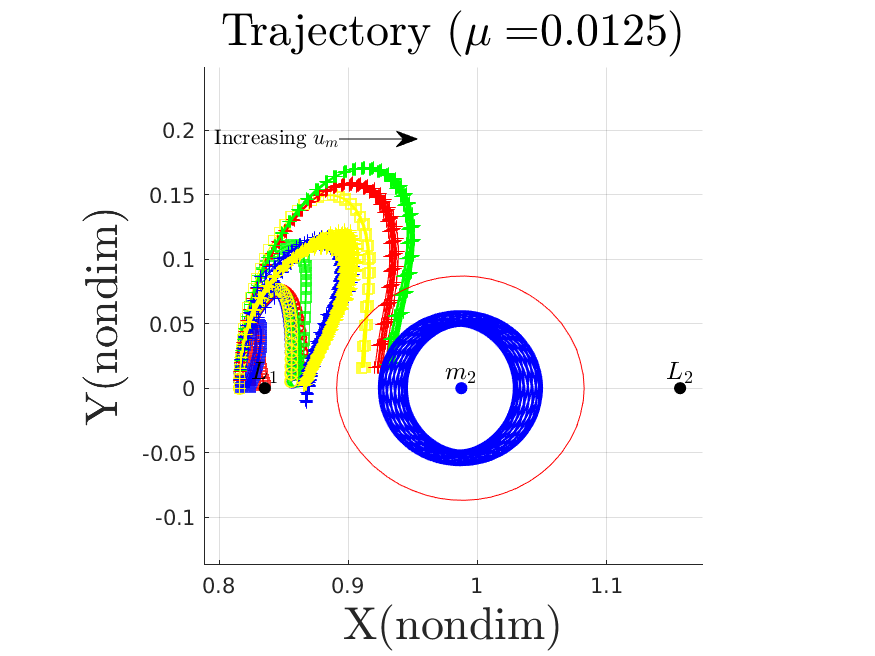
\includegraphics[width=0.5\textwidth]{figures/l1_transfer/trajectory_varying_um.pdf}}~
                \subcaptionbox{\Poincare section view of reachability sets}{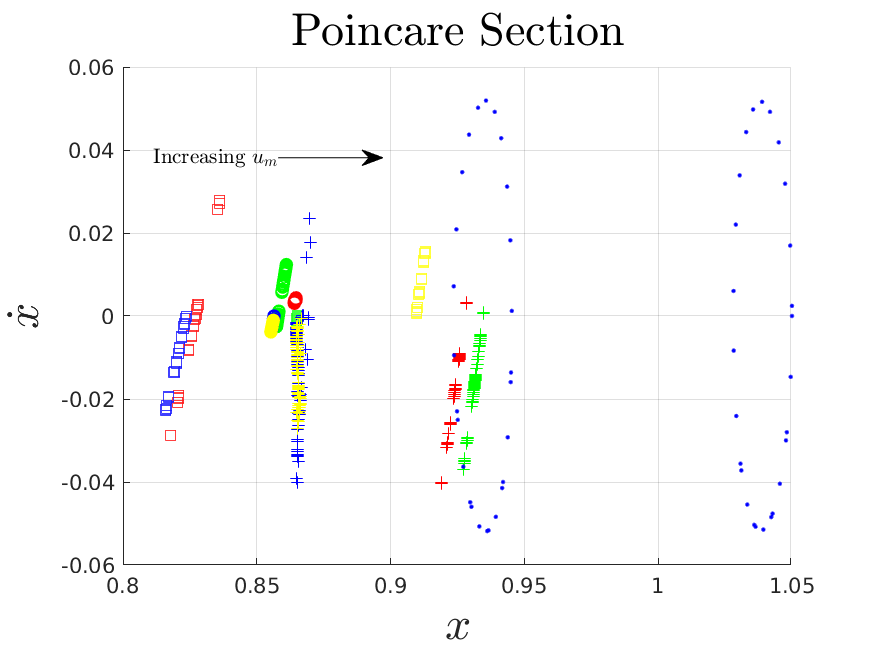
\includegraphics[width=0.5\textwidth]{figures/l1_transfer/poincare_section_varying_um.pdf}}
                \caption{Variation of \( t_f \) and \( u_m\) on the reachability set. 
                    Colors, \braces{red, blue, green, yellow}, are used note increasing \( t_f\) while markers, \braces{circle, square, cross}, are used to denote increasing \(u_m\).
                    Increasing the maximum control bound has a large effect and enables the reachability set to intersect the target manifold. 
                Increases in \(t_f\) are less critical and have minimal impact on the distribution of the reachability set on the \Poincare section.}
            \end{figure}

            \Cref{fig:varying_tf_reachability_sets} shows the reachabilty set for each combination of \(t_f\) and \( u_m\) listed in~\cref{tab:varying_tf}.
            Assuming a small control bound of \( u_m = \num{0.05} \) is shown in ~\cref{fig:varying_tf_reachability_sets} using square markers with the various terminal times shown using different colors.
            With a small maximum control bound, \( u_m = \num{0.05} \), the reachable set is not dramatically changed from that of the no control solution.
            The reachable set is shown using square markers on the left most portion of \cref{fig:varying_tf_poincare}.
            Variations of \( t_f\) are indicated using different colors and also demonstrate that this parameters has a smaller impact than changes in \( u_m \).
            Increasing the control bound to \( u_m = \num{0.25} \) and \( u_m = \num{0.5} \) shows that the reachable set is progressively approaching the target set and there are several intersections.

            The reachable sets presented in~\cref{fig:varying_tf_reachability_sets} are highly dependent on the initial condition, terminal time, and maximum control bound. 
            This example demonstrates that increasing the \( u_m \) results in a larger displacement between the controlled and uncontrolled trajectories.
            The reachable set is enlarged from a single point, as shown in~\cref{fig:manifold_poincare} by the black point, to a larger region as shown in~\cref{fig:varying_tf_poincare}.
            The choice of \( u_m\), \( t_f \) and initial condition all combine to change the resulting reachability set. 

        \end{correction}
    \item 
        \begin{itshape}
            The specification of a departure point from the periodic orbit.  In response to this question, the authors describe how the use of low-thrust propulsion enlarges the reachable set about some "center" defined by one branch of the uncontrolled manifold.  This is a key way to think about the approach you've posed but it is not illustrated in the paper.  Why not generate some curves under different thrust bounds for a specific departure point/manifold branch?  Again you'd be using a sidelined parameter to illustrate something fundamental about the approach.  And just maybe there would be a point at which, with high thrust, you start to see "bang-bang" type control and establish more connection to intuition.  
        \end{itshape}
    
        Thank you for the comment.
        We have included an additional section describing the effect of varaitions in \( u_m \) and terminal time on the reachable set.
        As discussed above, the results are not an exhaustive exploration of the parameter space but illustrate the key effect of the control bound and terminal time.
        In the example presented, increasing the magnitude of the control has the effect of enlarging and moving the reachable set. 
        At a sufficiently large value of \( u_m \) the reachable set is able to intersect the target orbit.

    \item 
        \begin{itshape}
            Actually, the influence of the starting point selection *is* somewhat illustrated by the green unstable manifold of Fig7b/8b.  The way a mission designer might think about applying this tool could be to start with this information as a baseline and then use principles revealed by the preceding two types of illustration to make some informed way of selecting a combination of [departure point, travel time, max thrust] to get the sets to intersect without oversizing their system.  That said, it's a little confusing how the red and green curves of Fig8b don't line up with this description to fit the comment of P18L47; additional consideration/analysis may be needed with regards to the number of revs/crossings used to define a section for comparison.
        \end{itshape}
        
        Thank you for the comment.
        As stated in the previous comments we have included additional discussion on the effect of variations of terminal time and control bound.

        \begin{itshape}
That said, it's a little confusing how the red and green curves of Fig8b don't line up with this description to fit the comment of P18L47; additional consideration/analysis may be needed with regards to the number of revs/crossings used to define a section for comparison.
        \end{itshape}
        
        Thank you for the question. 
        The green points are the intersection of the unstable manifold with the \Poincare section while the red points are the reachability set.
        Without any control input the spacecraft would remain on the periodic orbit and intersect the \Poincare seciton at \( x_n\). 
        The addition of the control input allows for an expansion of the reachable set from a single point to the larger red region.
        An additional clarification has been added to the manuscript to aid in the description of the figure.

        \begin{correction}
            In contrast, the low thrust control input we are able to enlarge the reachability set from a single point, \( x_n\) associated with the periodic orbit, to a larger ellipsoidal region shown in red in~\cref{fig:poincare_compare}.
        \end{correction}

    \item
        \begin{itshape}
            I previously mentioned my dissatisfaction with the interpretability of the control solution (which is plotted in planar components).  On further consideration, I think a time series plot of the Jacobi energy would be beneficial to help vet whether the method is working reasonably.  From intuition, one might expect an efficient solution to exhibit a span of monotonic energy increase, a relatively constant coasting span, and then a monotonic decrease back to the Poincare section value.  As is, the two roughly constant thrusting phases visible in the plot suggest that this might be happening, but it's hard to be sure.  Less consistent behavior might indicate, for example, that a longer-than-necessary transfer time was used.  
        \end{itshape}
        
        Additional plots have been included in the manuscript which shows the evolution of the Jacobi energy integral over the transfer horizon.
        
        The additional plot and some additional discussion for the first periodic orbit transfer is presented below.
        \begin{correction}
            \begin{figure} 
                \centering 
                \begin{subfigure}[htbp]{0.4\textwidth} 
                    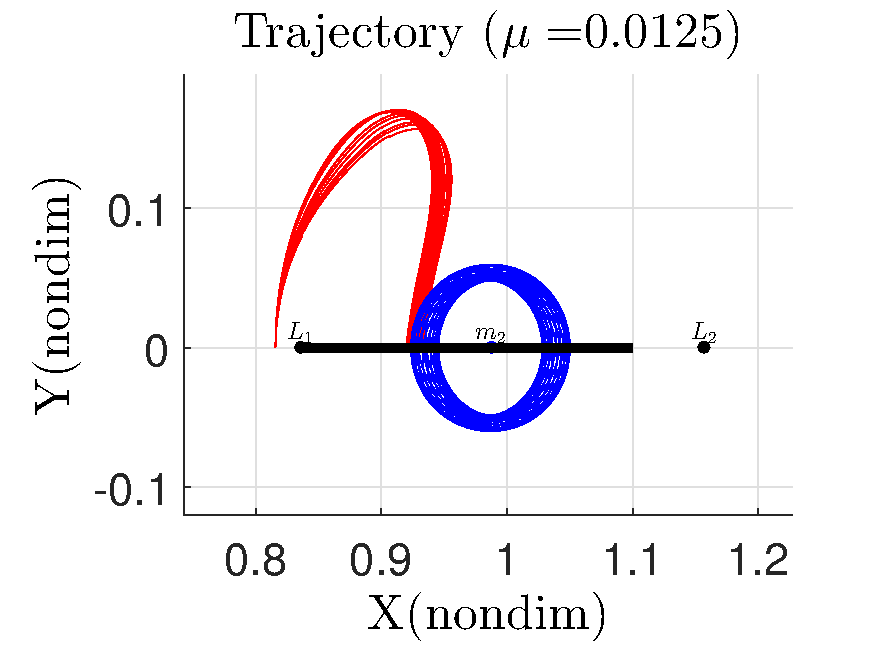
\includegraphics[width=\textwidth]{reach_trajectory} 
                    \caption{Position space view of reachability set} \label{fig:reach_trajectory} 
                \end{subfigure}~ %add desired spacing between images, e. g. ~, \quad, \qquad, \hfill etc. %(or a blank line to force the subfigure onto a new line) 
                \begin{subfigure}[htbp]{0.4\textwidth} 
                    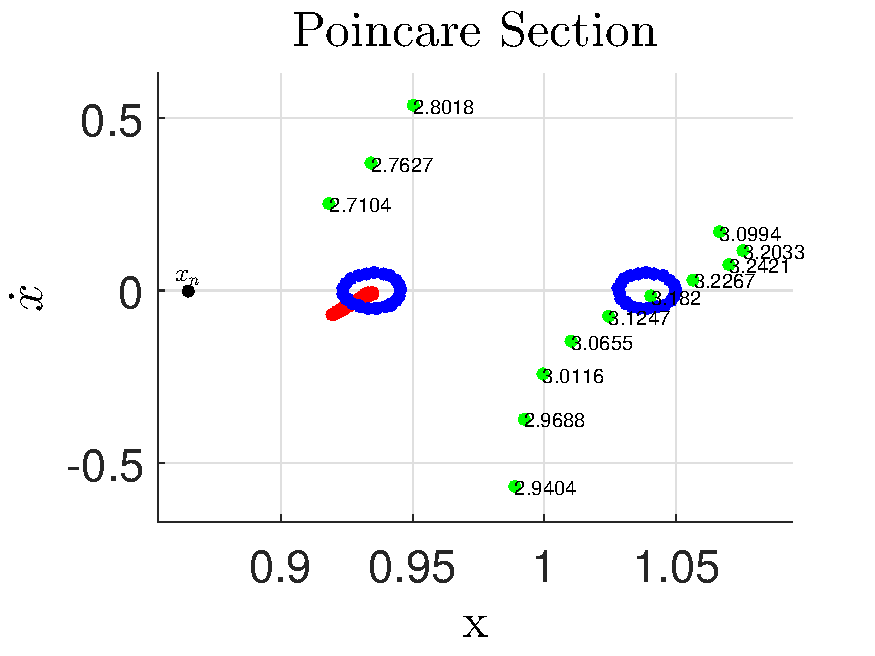
\includegraphics[width=\textwidth]{poincare_compare} 
                    \caption{\Poincare section view of reachability set} \label{fig:poincare_compare} 
                \end{subfigure} %add desired spacing between images, e. g. ~, \quad, \qquad, \hfill etc. %(or a blank line to force the subfigure onto a new line) 

                \begin{subfigure}[htbp]{0.4\textwidth} 
                    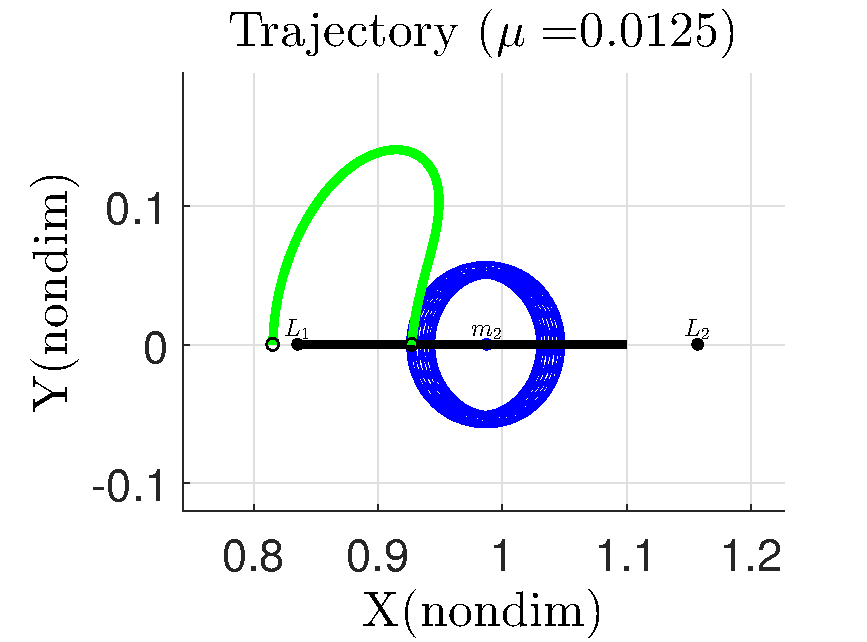
\includegraphics[width=\textwidth]{reach_transfer} 
                    \caption{Transfer trajectory selected from reachability set viewed in the position space} \label{fig:reach_transfer} 
                \end{subfigure}~ 
                \begin{subfigure}[htbp]{0.4\textwidth} 
                    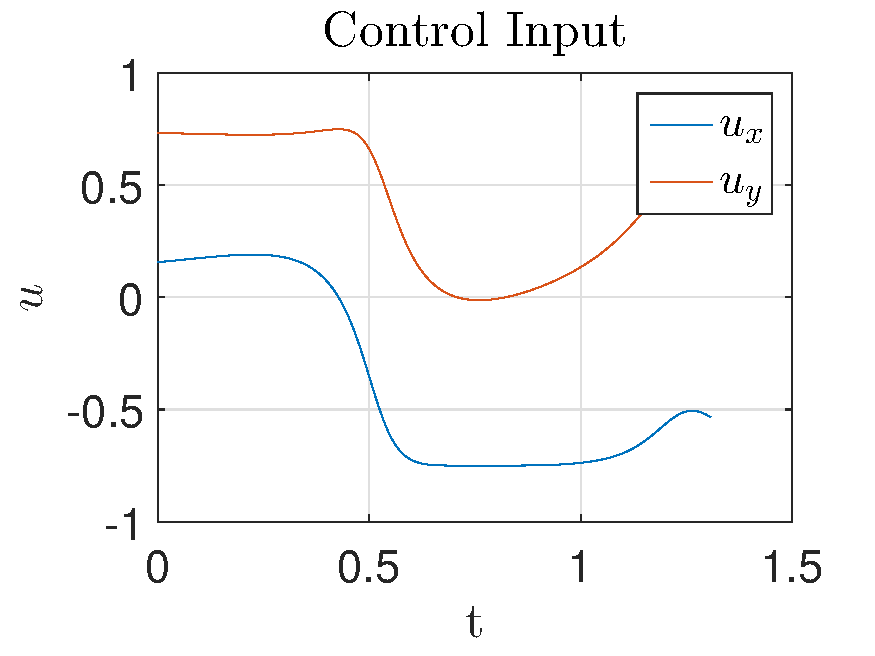
\includegraphics[width=\textwidth]{control_input_l1} 
                    \caption{Control input for the selected transfer trajectory} \label{fig:control_l1} 
                \end{subfigure}~

                \begin{subfigure}[htbp]{0.4\textwidth} 
                    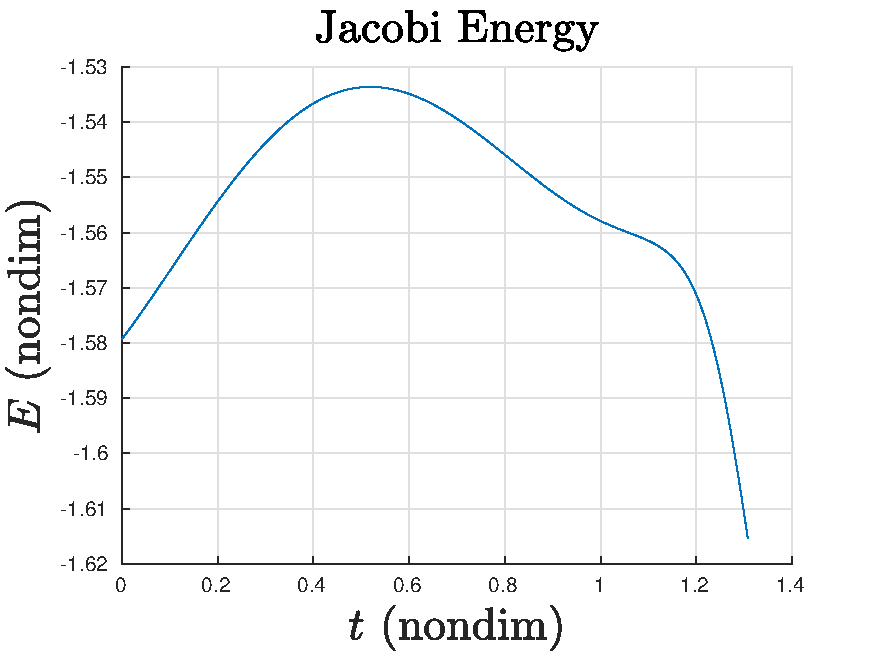
\includegraphics[width=\textwidth, keepaspectratio]{figures/l1_transfer/jacobi.pdf} 
                    \caption{Jacobi Energy over transfer \label{fig:jacobi_l1}} 
                \end{subfigure} 

                \caption{\( L_1 \) Reachability set transfer: The low thrust propulsion is used to approximate the reachability set starting from the initial periodic orbit over a fixed time horizon.
                    The reachability set is shown in the upper two figures in both the position and \Poincare space.
                    From this reachability set we chose a trajectory which intersects the target orbit and it is shown in the lower left figure.
                The optimal control to achieve this transfer is shown in the lower right figure.}
                \label{fig:reachability_set_transfer} 
            \end{figure}

            The Jacobi energy integral, computed using~\cref{eq:jacobi}, is shown in~\cref{fig:jacobi_l1}.
            \Cref{fig:jacobi_l1} shows that the vehicle begins with an energy level equal to the periodic orbit and arrives at the target orbit with the appropriate energy.
            The first half of the transfer is associated with and increase in energy as the control is used to transition towards the target orbit which is followed by a energy decrease to the target orbit.
            This roughly corresponds with the expected optimal solution of a bang-coast-bang type orbital transfer.

        \end{correction}
        The additional plot for the geostationary orbit transfer is presented below.
        \begin{correction}

Each stage of the transfer serves to raise the energy level of the vehicle.
After eight stages the reachability set intersects the stable manifold and a demonstrates that a transfer is achievable.
The final optimal control drives the vehicle towards the target manifold with the appropriate energy level.
\begin{figure} 
        \centering 
        \subcaptionbox{Transfer trajectory: Complete trajectory consisting of eight iterations (1-7 black and final in red) of the reachability sets with a final control-free coast (blue)  on the stable manifold (green).\label{fig:geo_transfer_full}}{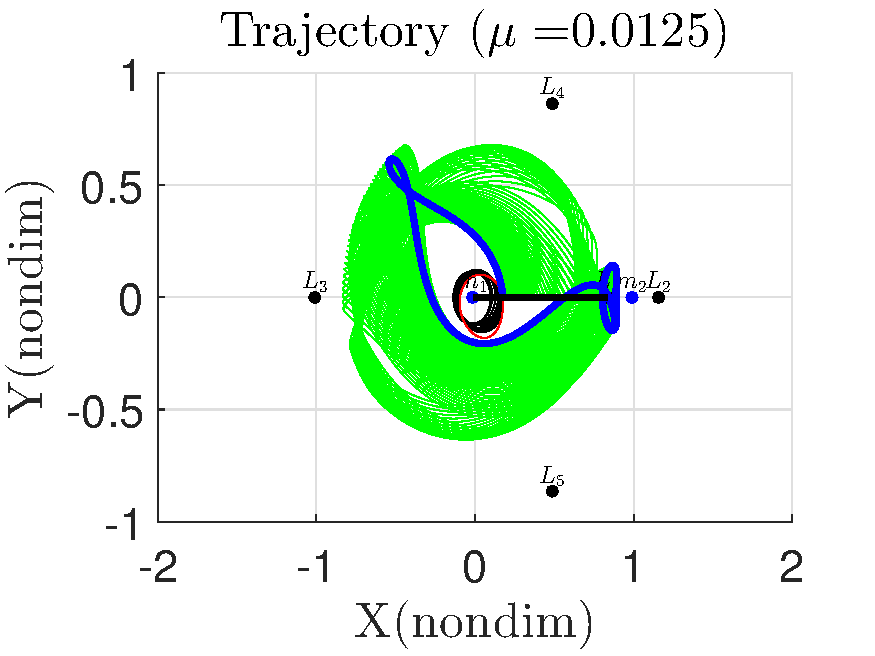
\includegraphics[width=0.4\textwidth]{geo_transfer_full}}\hfill
        \subcaptionbox{Detailed view of transfer: Centered at \(m_1\) the eight
            iterations from the reachability analysis are shown in black.  The
            final segment to the stable manifold is shown in red.  Each
            iteration progressively approaches the stable manifold.  Once on
        the stable manifold the vehicle can coast without thrust towards the
    periodic orbit.\label{fig:geo_transfer_zoom}
}{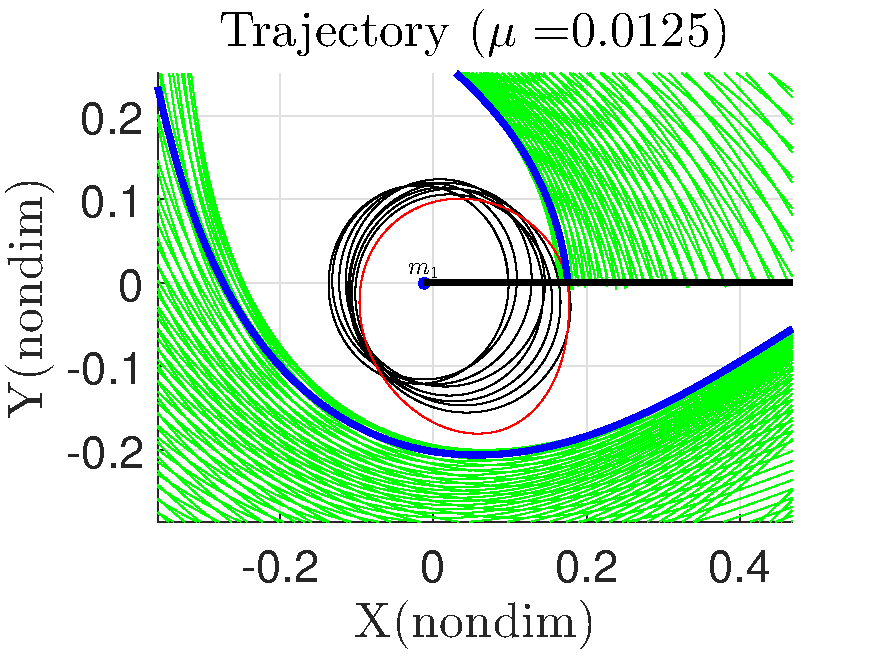
\includegraphics[width=0.4\textwidth]{geo_transfer_zoom}}
       
\subcaptionbox{\Poincare section: Minimum distance states from each iteration of the reachability set analysis (red) with respect to the stable invariant manifold (green)\label{fig:geo_transfer_poincare}}{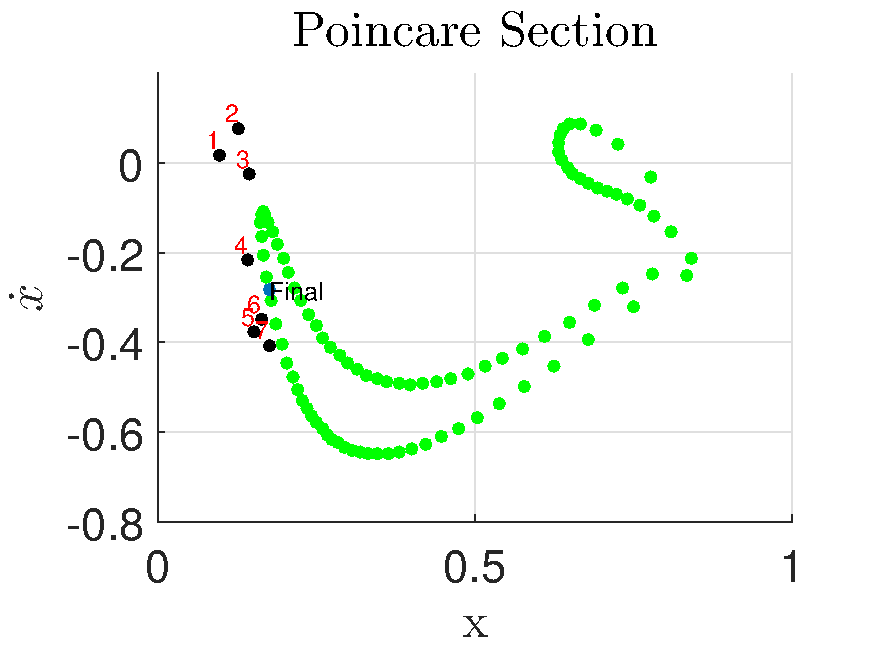
\includegraphics[width=0.4\textwidth]{poincare}}
    \hfill
    \subcaptionbox{Control Input: Combined control history for each stage of the reachability analysis. 
    The control always remains within the maximum bound.\label{fig:control_input_geo}}{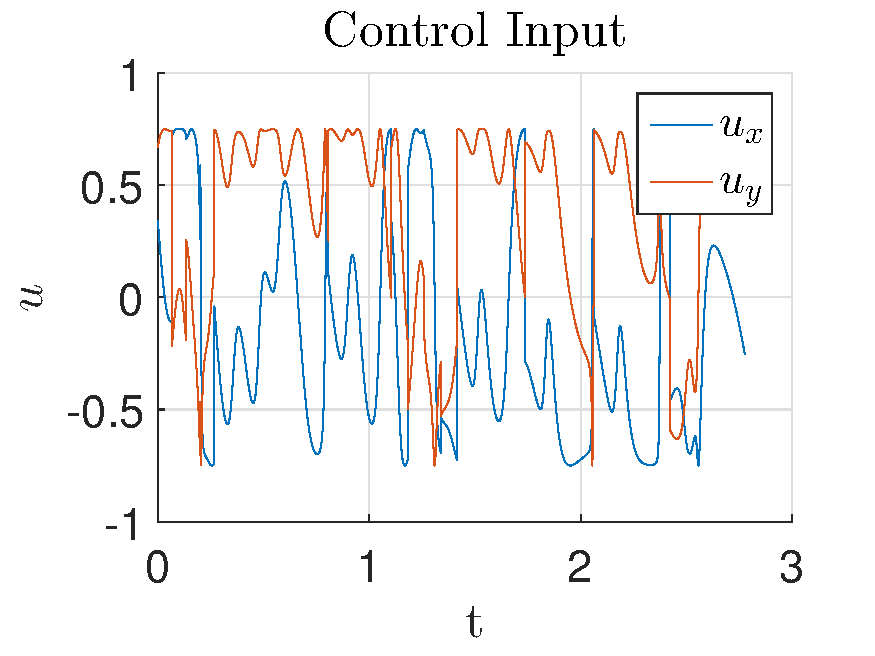
\includegraphics[width=0.4\textwidth]{figures/control_input_geo.pdf}}

    \subcaptionbox{Jacobi Energy: Energy history throughout the transfer.
    Each stage of the transfer serves to increase the energy towards the stable manifold. 
The final reachability set intersects the stable manifold and enables a large final manuever to the target orbit.\label{fig:jacobi_geo}}{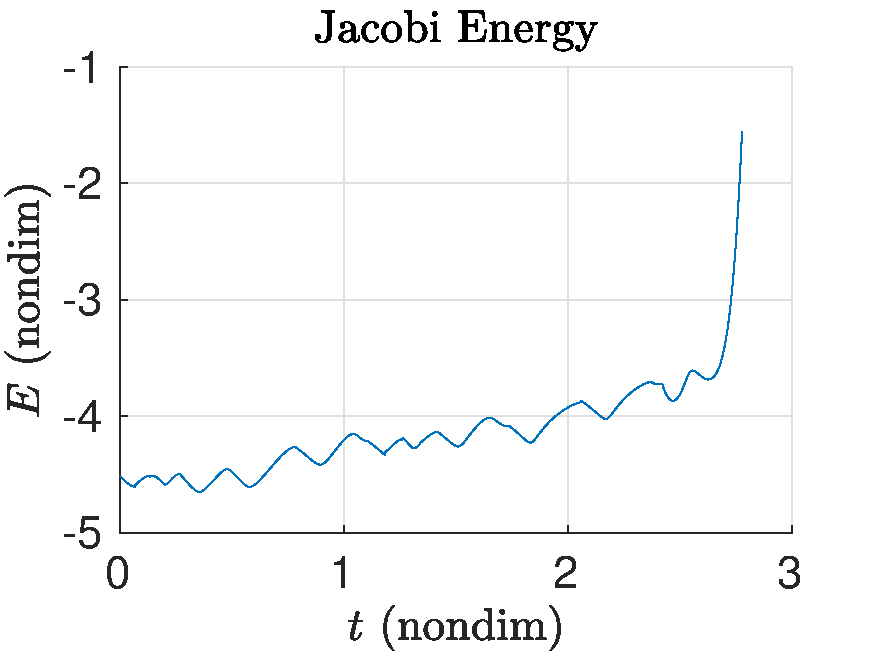
\includegraphics[width=0.4\textwidth]{figures/geo_transfer/jacobi_energy.pdf}}

        \caption{Geostationary to \( L_1 \) periodic orbit transfer: Complete transfer from the geostationary orbit to the stable manifold.\label{fig:geo_transfer}}
\end{figure}
        \end{correction}
    \item 
        \begin{itshape}
            Following that thought, I have serious concerns about chaining this Poincare-based approach, as done in the second problem and as I previously asked about.  The authors' responded: "While the trajectories do return to the energy level of the Poincare section, there is a transfer of "energy" between the states of the vehicle." Frankly, this statement doesn't make sense to me.  I think that you are actually getting a very inefficient solution by forcing these repeated (and at fixed intervals) returns to the same energy level (again, plot the Jacobi time series and see if you can square it with your intuition).  Furthermore posing the problem as a transfer to the stable manifold kind of hamstrings the motivation of reducing transfer times.  Honestly, I think this second example should simply be axed.  If the first one is expanded enough to illustrate the problem fundamentals, it will be sufficient.  Conducting the same kind of analysis at a couple different rev counts would
            reveal the dimension that this second example added, and help reveal the limits of the approach under certain scenarios and thrust capabilities.
        \end{itshape}

		As pointed out by the reviewer, our respond stating `..the trajectories do return to the energy level of the Poincare section..' is not correct. 
        Instead, the combination of several reachability sets does not force the system to return to a prescribed energy level.
        Each reachability set computation serves to maximize a distance metric, defined in a reduced phase space corresponding to the \Poincare section.
        The cost function is computed as the distance between the terminal states of the controlled and uncontrolled trajectories.
        The additional plots shown in both examples highlight the fact that the Jacobi energy is continuously changing as the control input is used to maneuver the vehicle towards the desired target states.

        The transfer to the stable manifold is presented as an example of the combination of existing control free  transfer methodologies with low thrust control inputs.
        This example demonstrates one possible use of low-thrust control to enable a larger region of feasibility for the use of invariant manifold transfers in the three body problem. 

		With regards to the comments on the second example, the authors decided to keep them in the manuscript, as it illustrates the idea of multiple stages to construct orbital maneuvers with more challenging scenarios. 
		Nonetheless, the revised manuscript includes extended numerical results and discussions for the first example, for example to illustrate the effects of varying $t_f$ and $u_m$ and the evolution of the Jacobi constant. 
    \item 
        \begin{itshape}
            To summarize my thoughts on ISSUE 2:
            As they exist, the examples illustrate that solutions can be found but they do not enlighten the reader as to the characteristics of the problem formulation/tool that should be understood and kept in mind when applying it or when planning related research efforts.  Furthermore, I am very suspicious that Example 2 is not actually a good solution or a compelling use case for the approach.  I do not necessarily ask or expect the authors to follow my above outline precisely, but I insist that some changes occur to make the analysis/illustrations better convey the general nature of the tool, not just that it gives you an answer.  
        \end{itshape}
    
        Thank you for the comments.
        The manuscript has been editied, as described previously, to incorporate several changes to illustrate the specific characteristics of this approach.
        An additional section is presented which highlights the effect of terminal time and control magnitude on the reachability set. 

        The second example presents a larger and more involved example of combining several iterations of the reachable set to achieve a larger and more complex transfer. 
        This aspect of the proposed method, more specifically of combining several reachability sets to approach a target, is not demonstrated in the first example.
        As a result, we feel that the second example does add some additional insight into the use of this method for a more complicated transfer.
		Furthermore, the revised conclusions section summarizes the objective of the submitted manuscript, and the pros and the cons of the proposed approach. 

    \item
        \begin{itshape}
            A more collected and focused discussion about how the parameter choices, assumptions, and limitations of the tool should inform its use is also warranted; currently remarks to this effect feel like scattered afterthoughts.  One organized way to think about this is to distinguish all the dimensions of the problem and identify what is being solved rigorously, what is being set manually, what is being numerically explored, etc.
        \end{itshape}

        Thank you for the helpful comments to improve the manuscript.
        The manuscript has been edited to reduce the length and repetition of the introduction.
        In addition, an additional section is presented highlighting the effect of the variations of terminal time and control magnitude on the reachable set. 
        Furthermore, the presented examples also include additional plots showing the change of the Jacobi energy during the transfer. 
\end{itemize}
% \bibliography{library}
% \bibliographystyle{spmpsci}
\end{document}

